\documentclass[extrafontsizes,60pt]{memoir}
\usepackage{amsmath,amssymb,amsfonts,amsthm}
\usepackage{lipsum}
\usepackage{fancyhdr}
\usepackage{xcolor}
\usepackage{hyperref} 
\usepackage{graphicx}
\usepackage[most]{tcolorbox}
\usepackage{tgpagella}
% \usepackage[p,osf]{scholax}
\usepackage[scaled=1.08,ncf,vvarbb]{newtxmath}
% \usepackage{beton}
% \usepackage{euler}
% \usepackage[OT1]{fontenc}

\everymath{\color{red}}
\everydisplay{\color{red}}

\usepackage[
margin = 1in,
paperwidth = 16in,
paperheight = 9in
]{geometry} 

\tolerance=1
\emergencystretch=\maxdimen
\hyphenpenalty=10000
\hbadness=10000

\providecommand{\tightlist}{%
  \setlength{\itemsep}{0pt}\setlength{\parskip}{0pt}}

\newcommand{\fonter}[1]{\fontsize{#1}{#1}\selectfont} 

\pagestyle{empty}
% \rfoot{\thepage/\lastpage}
\cfoot{}

\newtcolorbox{defn}[1]{
    enhanced, 
    frame hidden,
    colback=green,
    top=3mm,
    underlay={%
        \fill[orange!70, rounded corners] (frame.north west)--([shift={(5mm,5mm)}]frame.north east)--([shift={(2mm,-3mm)}]frame.south east) -- ([shift={(0mm,-1mm)}]frame.south west) -- cycle;
        \fill[white, rounded corners] (interior.north west) rectangle (interior.south east);},
    overlay={%
        \node[font=\sffamily\fonter{50pt}\bfseries, text=blue, anchor=west, rotate=0.7] at ([yshift=7mm] frame.north west) {#1};} 
}

\newenvironment{dbox}[1]
  {\begin{defn}{#1}}
  {\end{defn}}

\begin{document}
% \pagecolor{black}
% {\fontsize{8pt}{8pt}\selectfont \phantom{heheh}}
% \phatnom
\vspace{1mm}
\begin{center}
{\fonter{130pt}\bfseries Functions \& Relations}\\[150pt]
{\fonter{50pt} \bfseries\textcolor{blue}{Prof. Rey R. Cuenca}}\\
{\fonter{30pt} \textcolor{red}{DMS, MSU-IIT}}
\end{center}
\newpage

\clearpage

\begin{dbox}{Definition}
A \textbf{relation} \(R\) from the set \(X\) to a set \(Y\) is a rule that assigns to each element of \(X\) at least one element of \(Y\).

\end{dbox}

\fonter{60pt}
\begin{itemize}
 \item[] $X$ is called the \textit{\bfseries domain} of $R$
 \item[] $Y$ is called the \textit{\bfseries co-domain} of $R$
\end{itemize}

\newpage
\begin{center}
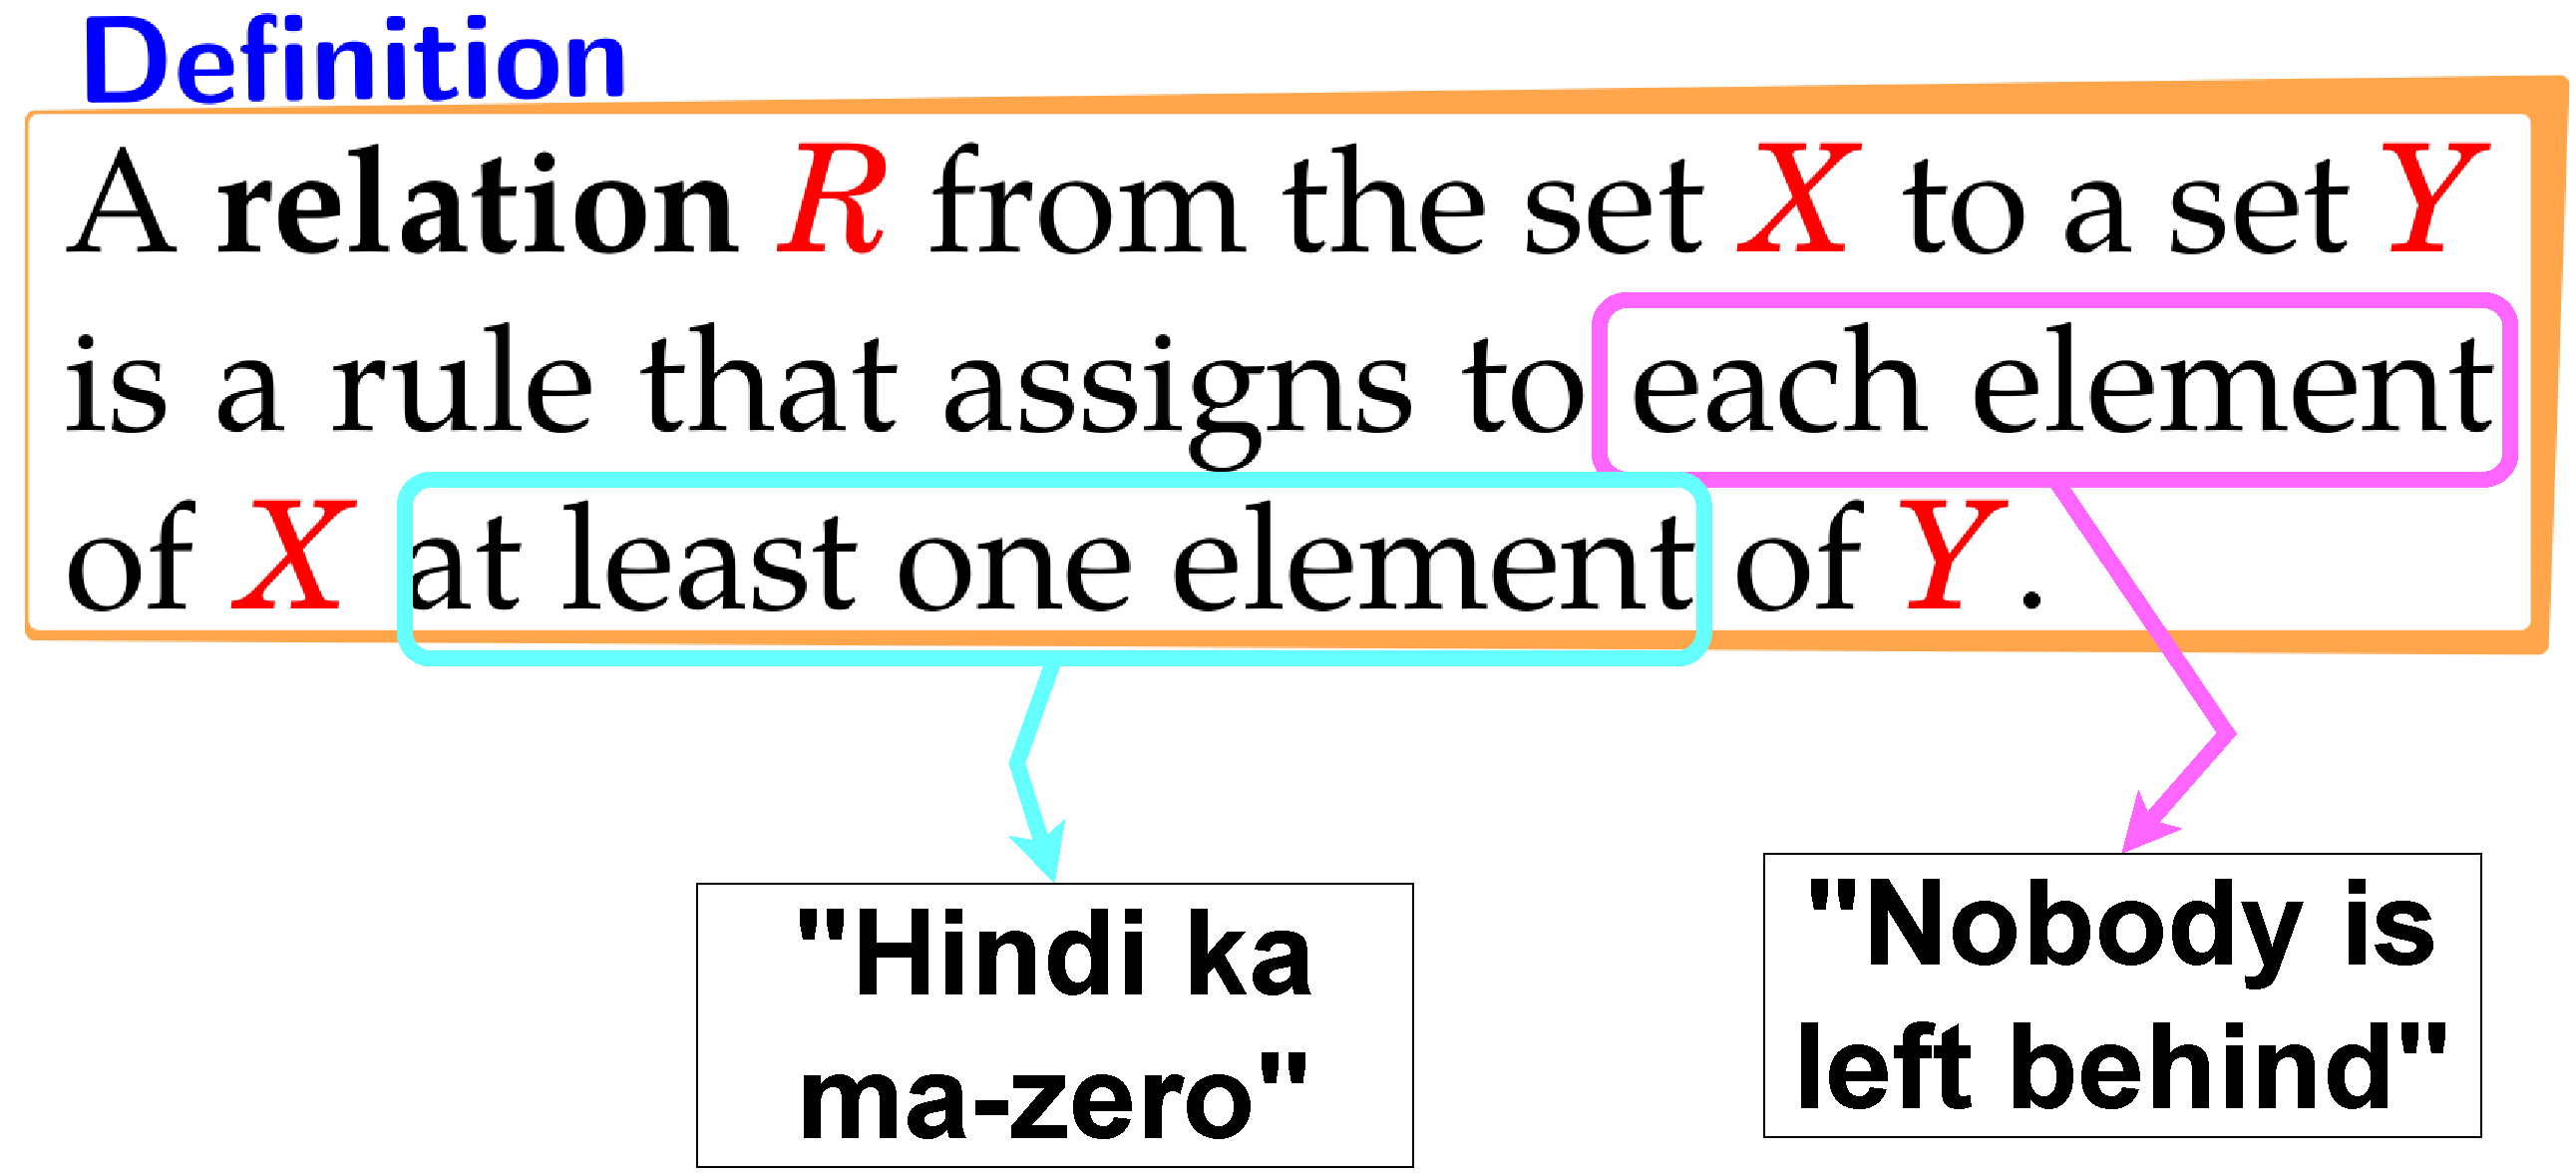
\includegraphics[width=\linewidth]{img/relations-slide-01-annotation.pdf}
\end{center}
\newpage

\begin{dbox}{Definition}
The \textbf{range} of a relation \(R\) is the set of all elements in the co-domain \(Y\) that is assigned to some element in the domain \(X\).

\end{dbox}
\end{document}
